\documentclass[11pt]{article}
\usepackage{spikey}
\usepackage{amsmath}
\usepackage{amssymb}
\usepackage{soul}
\usepackage{float}
\usepackage{graphicx}
\usepackage{hyperref}
\usepackage{xcolor}
\usepackage{chngcntr}
\usepackage{centernot}
\usepackage{datetime}
\usepackage[shortlabels]{enumitem}

\usepackage[margin=1truein]{geometry}
\usepackage{setspace}
\linespread{1.15}

\counterwithin{equation}{section}
\newcommand{\upi}[0]{^{(i)}}

\title{CS229 Problem Set 1}
\date{\today}
\author{Tianyu Du}
\begin{document}
	\maketitle
	\newpage
	\section{Question 1: Linear Classifiers}
	\subsection{Question 1(a)}
	\begin{lemma}
		\begin{equation}
			g'(z) = g(z) \left(1-g(z)\right)
		\end{equation}
	\end{lemma}
	
	\begin{lemma} For every $x, z \in \R^n$,
		\begin{equation}
			\sum_i \sum_j z_i x_i z_j x_j = (x^T z)^2 \geq 0
		\end{equation}
	\end{lemma}
	
	\begin{align}
		\nabla_\theta J(\theta) &= - \frac{1}{n} \sum_{i=1}^n \left(
		y\upi \frac{g'(\theta^T x\upi)}{g(\theta^T x\upi)}
		- (1 - y\upi) \frac{g'(\theta^T x\upi)}{1-g(\theta^T x\upi)}
		\right) x\upi \\
		&= - \frac{1}{n} \sum_{i=1}^n \left(
		y\upi (1 - g(\theta^T x\upi)) - (1 - y\upi) g(\theta^T x\upi)
		\right) x\upi \\
		&= - \frac{1}{n} \sum_{i=1}^n \left(
		y\upi - g(\theta^T x\upi)
		\right ) x\upi \\
		\implies \pd{J(\theta)}{\theta_j} &= - \frac{1}{n} \sum_{i=1}^n \left(
		y\upi - g(\theta^T x\upi)
		\right ) x\upi_j\ \forall j \in [d]\\
		\implies \forall k \in [d],\ \frac{\partial^2 J(\theta)}{\partial \theta_j \partial \theta_k} &= -\frac{1}{n}\sum_{i=1}^n \left (
		- g(\theta^T x\upi) (1-g(\theta^T x\upi)) x\upi_k
		\right) x\upi_j \\
		&= \frac{1}{n}\sum_{i=1}^n \left (
		g(\theta^T x\upi) (1-g(\theta^T x\upi)) x\upi_j x\upi_k
		\right)
	\end{align}
	Therefore, $H_J (\theta)$ can be constructed from the array of second order derivatives of $J(\theta)$ as 
	\begin{equation}
		H_J(\theta)_{j, k} := \frac{1}{n}\sum_{i=1}^n \left (
		g(\theta^T x\upi) (1-g(\theta^T x\upi)) x\upi_j x\upi_k
		\right)
	\end{equation}
	Notice that since $g(\theta^T x\upi) \in (0, 1)$, therefore $g(\theta^T x\upi) (1-g(\theta^T x\upi)) > 0$ for every $\theta$ and $x\upi$.
	\begin{proof} Show that $H_J (\theta) \succeq 0$: let $z = (z_1,\dots,z_d) \in \R^d$, then
		\begin{align}
			z^T H_J (\theta) \in \R^{1 \times d}
		\end{align}
		Then the $\beta^{th}$ column of $z^T H_J (\theta)$ is
		\begin{align}
			z^T H_J (\theta)_{\beta} &= \frac{1}{n} \sum_{\alpha=1}^d \sum_{i=1}^n g(\theta^T x\upi) (1-g(\theta^T x\upi)) z_\alpha x\upi_\alpha x\upi_\beta
		\end{align}
		Therefore
		\begin{align}
			z^T H_J(\theta) z &= \frac{1}{n} \sum_{\beta=1}^d \sum_{\alpha=1}^d \sum_{i=1}^n g(\theta^T x\upi) (1-g(\theta^T x\upi)) z_\alpha x\upi_\alpha x\upi_\beta z_\beta \\
			&= \frac{1}{n} \sum_{i=1}^n g(\theta^T x\upi) (1-g(\theta^T x\upi)) \sum_{\beta=1}^d \sum_{\alpha=1}^d z_\alpha x\upi_\alpha x\upi_\beta z_\beta \\
			&= \frac{1}{n} \sum_{i=1}^n \underbrace{g(\theta^T x\upi) (1-g(\theta^T x\upi))}_{> 0\ \because g(\cdot) \in (0, 1)} \underbrace{(z^T x)^2}_{\geq 0} \geq 0
		\end{align}
		Hence, $H_J(\theta) \succeq 0$ is shown by showing $z^T H_J(\theta) z$ for every $z \in \R^d$.
	\end{proof}
	
	\newpage
	\subsection{Question 1(b) Coding}
	\begin{figure}[h]
		\centering
		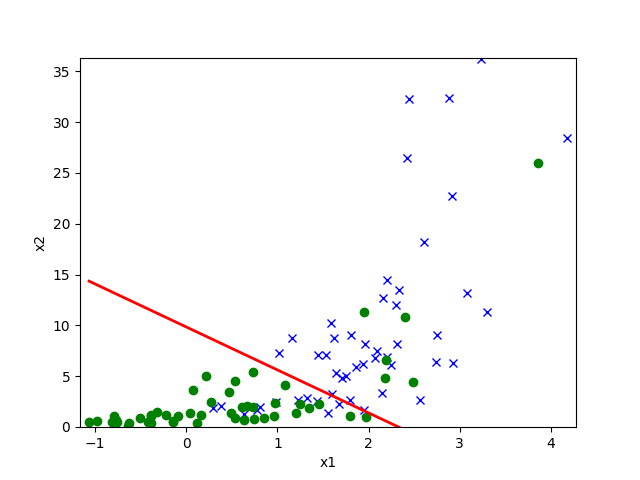
\includegraphics[width=0.6\linewidth]{src/linearclass/logreg_pred_1.png}
		\caption{Logistic Regression Decision Boundary on Dataset 1}
	\end{figure}
	
	\begin{figure}[h]
		\centering
		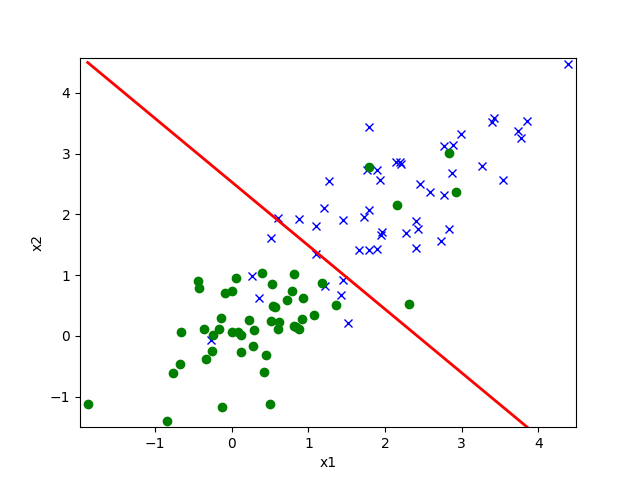
\includegraphics[width=0.6\linewidth]{src/linearclass/logreg_pred_2.png}
		\caption{Logistic Regression Decision Boundary on Dataset 2}
	\end{figure}
	
	
	\newpage
	\subsection{Question 1(c)}
	\begin{proof}
		By Bayes' theorem,
		\begin{align}
			p(y=1|x; \phi, \mu_0, \mu_1, \Sigma) &= \frac{p(x|y=1; \phi, \mu_0, \mu_1, \Sigma) p(y=1; \phi, \mu_0, \mu_1, \Sigma)}{p(x;\phi, \mu_0, \mu_1, \Sigma)}
		\end{align}
		Define 
		\begin{align}
			z &:= \frac{p(x|y=1; \phi, \mu_0, \mu_1, \Sigma) p(y=1; \phi, \mu_0, \mu_1, \Sigma)}{p(x;\phi, \mu_0, \mu_1, \Sigma)} \\
			\Theta &:= \{\phi, \mu_0, \mu_1, \Sigma\}
		\end{align}
		Conditioned on particular $x$, $y$ is either 0 or 1, therefore,
		\begin{align}
			p(y=0|x; \Theta) &= 1 - z \\
			\implies \frac{z}{1-z} &= \frac{p(y=1|x; \Theta)}{p(y=0|x; \Theta)} \\
			&= \frac{p(x|y=1; \Theta) p(y=1; \Theta)}{p(x|y=0; \Theta) p(y=0; \Theta)} \\
			&= \frac{\phi}{1 - \phi} \frac{\exp\left(-\frac{1}{2} (x-\mu_1)^T \Sigma^{-1} (x - \mu_1)\right)}{\exp\left(-\frac{1}{2} (x-\mu_0)^T \Sigma^{-1} (x - \mu_0)\right)} \\
			\implies \log \frac{z}{1-z} &= \log \frac{\phi}{1-\phi} \\
			&+ \left (-\frac{1}{2} x^T \Sigma^{-1} x + \mu_1^T \Sigma^{-1} x - \frac{1}{2} \mu_1^T \Sigma^{-1} \mu_1 \right) \\
			&- \left (-\frac{1}{2} x^T \Sigma^{-1} x + \mu_0^T \Sigma^{-1} x - \frac{1}{2} \mu_0^T \Sigma^{-1} \mu_0 \right) \\
			&= \log \frac{\phi}{1-\phi} + \left (
			(\mu_1 - \mu_0)^T \Sigma^{-1} x
			+ \frac{1}{2} \mu_0^T \Sigma^{-1} \mu_0 - \frac{1}{2} \mu_1^T \Sigma^{-1} \mu_1
			\right ) \\
			\implies \frac{z}{1-z} &= \exp \underbrace{\left (
			\log \frac{\phi}{1-\phi} + \left (
			(\mu_1 - \mu_0)^T \Sigma^{-1} x
			+ \frac{1}{2} \mu_0^T \Sigma^{-1} \mu_0 - \frac{1}{2} \mu_1^T \Sigma^{-1} \mu_1
			\right )
			\right )}_{=:\Delta} \\
			\implies z &= \frac{\exp(\Delta)}{1+\exp(\Delta)} = \frac{1}{1+\exp(-\Delta)}
		\end{align}
		Therefore
		\begin{align}
			\frac{p(x|y=1; \phi, \mu_0, \mu_1, \Sigma) p(y=1; \phi, \mu_0, \mu_1, \Sigma)}{p(x;\phi, \mu_0, \mu_1, \Sigma)}
			&= \frac{1}{1 + \exp(-(\theta^T x + \theta_0))}
		\end{align}
		where 
		\begin{align}
			\theta &= (\Sigma^{-1})^T (\mu_1 - \mu_0) \\
			\theta_0 &= \log \frac{\phi}{1-\phi} + \frac{1}{2} \mu_0^T \Sigma^{-1} \mu_0 - \frac{1}{2} \mu_1^T \Sigma^{-1} \mu_1
		\end{align}
	\end{proof}
	\newpage
	\subsection{Question 1(d)}
	\subsubsection{$\phi$}
	\begin{proof}
	\begin{align}
		\pd{}{\phi} \ell (\phi, \cdot) &= \pd{}{\phi} \sum_{i=1}^n
		\underbrace{\log p(x\upi|y\upi; \mu_0, \mu_1, \Sigma)}_{\perp \phi}
		+ \log p(y\upi; \phi) \\
		&= \pd{}{\phi} \sum_{i=1}^n \log p(y\upi; \phi) \\
		&= \pd{}{\phi} \sum_{i=1}^n \log \phi^{y\upi} (1 - \phi)^{1 - y\upi} \\
		&= \pd{}{\phi} \sum_{i=1}^n y\upi \log \phi + (1 - y\upi) \log (1 - \phi) \\
		&= \sum_{i=1}^n y\upi \frac{1}{\phi} - (1 - y\upi) \frac{1}{1 - \phi}
	\end{align}
	The first order condition of maximizing likelihood becomes
	\begin{align}
		\sum_{i=1}^n y\upi \frac{1}{\phi} - (1 - y\upi) \frac{1}{1 - \phi} &= 0 \\
		\implies \sum_{i=1} \frac{y\upi}{\phi} + \frac{y\upi}{1 - \phi} - \frac{1}{1 - \phi} &= 0 \\
		\implies \sum_{i=1}^n y\upi \frac{1 - \phi + \phi}{\phi (1 - \phi)} - \frac{1}{1 - \phi} &= 0 \\
		\implies \sum_{i=1}^n y\upi \frac{1}{\phi (1 - \phi)} &= n \frac{1}{1-\phi} \\
		\implies \phi &= \frac{1}{n} \sum_{i=1}^n y\upi
	\end{align}
	\end{proof}
	
	\subsubsection{$\mu_0$}
	\begin{proof}
		\begin{align}
			\pd{}{\mu_0} \ell(\mu_0, \cdot) &= \pd{}{\mu_0} \sum_{i=1}^n
		\log p(x\upi|y\upi; \mu_0, \mu_1, \Sigma)
		+ \underbrace{\log p(y\upi; \phi)}_{\perp \mu_0} \\
		&= \pd{}{\mu_0} \sum_{i=1}^n \log p(x\upi|y\upi; \mu_0, \mu_1, \Sigma) \\
		&= \pd{}{\mu_0} \sum_{i=1}^n \Big\{
		\overbrace{
		y\upi \log \left [ \frac{1}{(2\pi)^{d/2}|\Sigma|^{1/2}} \exp \left (-\frac{1}{2} (x\upi - \mu_1)^T \Sigma^{-1} (x\upi - \mu_1) \right) \right ]}^{\perp \mu_0} \\
		&+ (1 - y\upi) \log \left [ \frac{1}{(2\pi)^{d/2}|\Sigma|^{1/2}} \exp \left (-\frac{1}{2} (x\upi - \mu_0)^T \Sigma^{-1} (x\upi - \mu_0) \right) \right ] \Big\} \\
		&= \pd{}{\mu_0} \sum_{i=1}^n (1 - y\upi) \left (
		\underbrace{\log \frac{1}{(2\pi)^{d/2}|\Sigma|^{1/2}}}_{\perp \mu_0}
		-\frac{1}{2} (x\upi - \mu_0)^T \Sigma^{-1} (x\upi - \mu_0) \right) \\
		&= \pd{}{\mu_0} (-1) \sum_{i=1}^n (1 - y\upi) \frac{1}{2} (x\upi - \mu_0)^T \Sigma^{-1} (x\upi - \mu_0) = 0 \\
		&\implies \sum_{i=1}^n (1 - y\upi) \Sigma^{-1} (x\upi - \mu_0) = 0 \\ \\
		&\implies \sum_{i=1}^n \Sigma^{-1} (1 - y\upi) x\upi = \sum_{i=1}^n \Sigma^{-1} (1 - y\upi) \mu_0 \\
		& \implies \sum_{i=1}^n (1 - y\upi) x\upi = \sum_{i=1}^n (1 - y\upi) \mu_0 \\
		& \implies \mu_0 = \frac{\sum_{i=1}^n (1 - y\upi) x\upi}{\sum_{i=1}^n (1 - y\upi)} = \frac{\sum_{i=1}^n \id{y\upi = 0} x\upi}{\sum_{i=1}^n \id{y\upi = 0}}
	\end{align}
	\end{proof}
	
	\subsubsection{$\mu_1$}
	\begin{proof}
		\begin{align}
			\pd{}{\mu_1} \ell(\mu_1, \cdot) &= \pd{}{\mu_1} \sum_{i=1}^n
		\log p(x\upi|y\upi; \mu_0, \mu_1, \Sigma)
		+ \underbrace{\log p(y\upi; \phi)}_{\perp \mu_1} \\
		&= \pd{}{\mu_1} \sum_{i=1}^n \log p(x\upi|y\upi; \mu_0, \mu_1, \Sigma) \\
		&= \pd{}{\mu_1} \sum_{i=1}^n \Big\{
		y\upi \log \left [ \frac{1}{(2\pi)^{d/2}|\Sigma|^{1/2}} \exp \left (-\frac{1}{2} (x\upi - \mu_1)^T \Sigma^{-1} (x\upi - \mu_1) \right) \right ] \\
		&+\underbrace{ (1 - y\upi) \log \left [ \frac{1}{(2\pi)^{d/2}|\Sigma|^{1/2}} \exp \left (-\frac{1}{2} (x\upi - \mu_0)^T \Sigma^{-1} (x\upi - \mu_0) \right) \right ]}_{\perp \mu_1}
		\Big\} \\
		&= \pd{}{\mu_1} \sum_{i=1}^n y\upi \left (
		\underbrace{\log \frac{1}{(2\pi)^{d/2}|\Sigma|^{1/2}}}_{\perp \mu_1}
		-\frac{1}{2} (x\upi - \mu_1)^T \Sigma^{-1} (x\upi - \mu_1) \right) \\
		&= \pd{}{\mu_1} (-1) \sum_{i=1}^n y\upi \frac{1}{2} (x\upi - \mu_1)^T \Sigma^{-1} (x\upi - \mu_1) = 0 \\
		&\implies \sum_{i=1}^n y\upi \Sigma^{-1} (x\upi - \mu_1) = 0 \\
		&\implies \sum_{i=1}^n \Sigma^{-1} y\upi x\upi = \sum_{i=1}^n \Sigma^{-1} y\upi \mu_1 \\
		& \implies \sum_{i=1}^n y\upi x\upi = \sum_{i=1}^n y\upi \mu_1 \\
		& \implies \mu_1 = \frac{\sum_{i=1}^n y\upi x\upi}{\sum_{i=1}^n y\upi} = \frac{\sum_{i=1}^n \id{y\upi = 1} x\upi}{\sum_{i=1}^n \id{y\upi = 1}}
	\end{align}
	\end{proof}
	
	\subsubsection{$\Sigma^{-1}$}
	\begin{lemma}
		Given matrices $A, B$ such that $AB$ and $BA$ are squared, then
		\begin{equation}
			\tx{tr}(AB) = \tx{tr}(BA)
		\end{equation}
		\begin{proof}
			In lecture notes.
		\end{proof}
	\end{lemma}
	
	\begin{lemma}
		\begin{align}
			\pd{}{A} \tx{tr}(AB) = \pd{}{A} \tx{tr}(BA) = B^T
		\end{align}
		\begin{proof}
			Let $A \in \R^{n \times m}$ and $B \in \R^{m \times n}$. Let $a_i \in \R^m$ denote the $i^{th}$ \ul{row} of matrix $A$, let $b_j \in \R^m$ denote the $j^{th}$ \ul{column} of matrix $B$,
			\begin{align}
				\tx{tr}(AB) &= \tx{tr}
				\begin{pmatrix}
					a_1 \cdot b_1 & a_1 \cdot b_2 & \cdots & a_1 \cdot b_n \\
					a_2 \cdot b_1 & a_2 \cdot b_2 & \cdots & a_2 \cdot b_n \\
					\vdots & & \ddots & \vdots \\
					a_n \cdot b_1 & a_n \cdot b_2 & \cdots & a_n \cdot b_n 
				\end{pmatrix} \\
				&= \sum_{i=1}^n a_i \cdot b_i \\
				&= \sum_{i=1}^n A_{i, j} B_{j, i} \\
				&\implies \pd{\tx{tr}(AB)}{A_{i,j}} = B_{j,i} \\
				&\implies \nabla_A \tx{tr}(AB) = B^T
			\end{align}
			Since $\tx{tr}(AB) = \tx{tr}(BA)$, $\nabla_A \tx{tr}(BA) = B^T$ as well.
		\end{proof}
	\end{lemma}
	
	\begin{proof}
		\begin{align}
			&\pd{}{\Sigma} \ell(\Sigma, \cdot) = 0 \\
			&\implies \pd{}{\Sigma} \sum_{i=1}^n \log(p(x\upi|y\upi;\mu_0, \mu_1, \Sigma)) 
			+ \underbrace{\log(p(y\upi;\phi))}_{\perp \Sigma} = 0 \\
			&\iff \pd{}{\Sigma} \sum_{i=1}^n \log(p(x\upi|y\upi;\mu_0, \mu_1, \Sigma)) = 0 \\
			&\implies 
			\pd{}{\Sigma} \sum_{i=1}^n y\upi \left [
				-\frac{d}{2} \log(2\pi) - \frac{1}{2} \log(|\Sigma|) - \frac{1}{2} (x\upi - \mu_1)^T \Sigma^{-1} (x\upi - \mu_1)
			\right ] \\
			&+ (1 - y\upi) \left [
				-\frac{d}{2} \log(2\pi) - \frac{1}{2} \log(|\Sigma|) - \frac{1}{2} (x\upi - \mu_0)^T \Sigma^{-1} (x\upi - \mu_0)
			\right ] = 0
		\end{align}
		where $-\frac{d}{2} \log(2\pi)$ is constant and independent from $\Sigma$, therefore it can be dropped in the first order condition.
		\begin{align}
			&\implies \pd{}{\Sigma} \sum_{i=1}^n y\upi \left [- \frac{1}{2} \log(|\Sigma|) - \frac{1}{2} (x\upi - \mu_1)^T \Sigma^{-1} (x\upi - \mu_1)
			\right ] \\
			&+ (1 - y\upi) \left [- \frac{1}{2} \log(|\Sigma|) - \frac{1}{2} (x\upi - \mu_0)^T \Sigma^{-1} (x\upi - \mu_0)
			\right ] = 0 \\
			&\implies \pd{}{\Sigma} \sum_{i=1}^n - \frac{1}{2} \log(|\Sigma|) - \frac{y\upi}{2} (x\upi - \mu_1)^T \Sigma^{-1} (x\upi - \mu_1) - \frac{1-y\upi}{2} (x\upi - \mu_0)^T \Sigma^{-1} (x\upi - \mu_0) = 0 \\
			&\implies \pd{}{\Sigma} \sum_{i=1}^n \log(|\Sigma|) 
			+ y\upi (x\upi - \mu_1)^T \Sigma^{-1} (x\upi - \mu_1) 
			+ (1-y\upi) (x\upi - \mu_0)^T \Sigma^{-1} (x\upi - \mu_0) = 0 \\
			&\implies n \Sigma^{-1} + \pd{}{\Sigma} \sum_{i=1}^n y\upi \tx{tr}((x\upi - \mu_1)^T \Sigma^{-1} (x\upi - \mu_1))
			+ (1-y\upi) \tx{tr}((x\upi - \mu_0)^T \Sigma^{-1} (x\upi - \mu_0)) = 0 \\
			&\implies n \Sigma^{-1} + \pd{}{\Sigma} \sum_{i=1}^n y\upi 
			\tx{tr}(
				\Sigma^{-1} (x\upi - \mu_1) (x\upi - \mu_1)^T
			)
			+ (1 - y\upi) 
			\tx{tr}(
				\Sigma^{-1} (x\upi - \mu_0) (x\upi - \mu_0)^T
			) = 0 \\
			&\implies n \Sigma^{-1} + \sum_{i=1}^n y\upi (x\upi - \mu_1) (x\upi - \mu_1)^T + (1 - y\upi) (x\upi - \mu_0) (x\upi - \mu_0)^T = 0 \\
			&\implies n \Sigma^{-1} + \sum_{i=1}^n (x\upi - \mu_{y\upi}) (x\upi - \mu_{y\upi})^T = 0 \\
			&\implies \Sigma = \frac{1}{n} \sum_{i=1}^n (x\upi - \mu_{y\upi}) (x\upi - \mu_{y\upi})^T \in \R^{d \times d}
		\end{align}
	\end{proof}
	
	\newpage
	\subsection{Question 1(e) Coding}
	\begin{figure}[h]
		\centering
		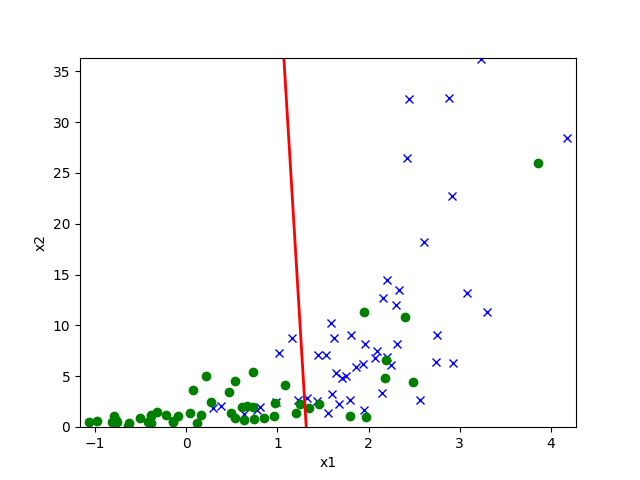
\includegraphics[width=0.6\linewidth]{src/linearclass/gda_pred_1.png}
		\caption{GDA Decision Boundary on Dataset 1}
	\end{figure}
	
	\begin{figure}[h]
		\centering
		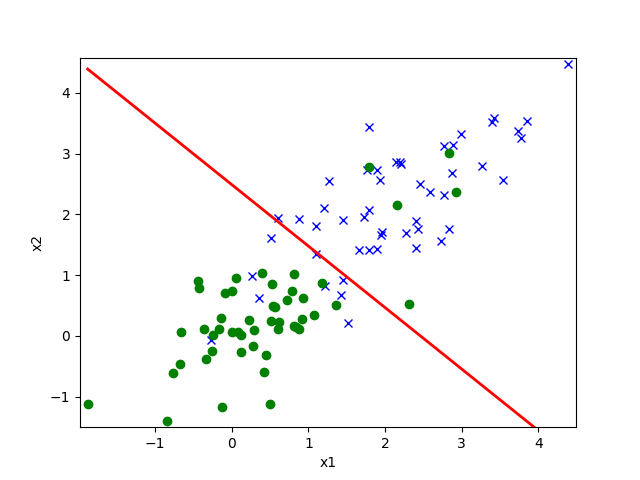
\includegraphics[width=0.6\linewidth]{src/linearclass/gda_pred_2.png}
		\caption{GDA Decision Boundary on Dataset 2}
	\end{figure}
	
	\newpage
	\subsection{Question 1 (f)}
%	\begin{figure}[h]
%		\centering
%		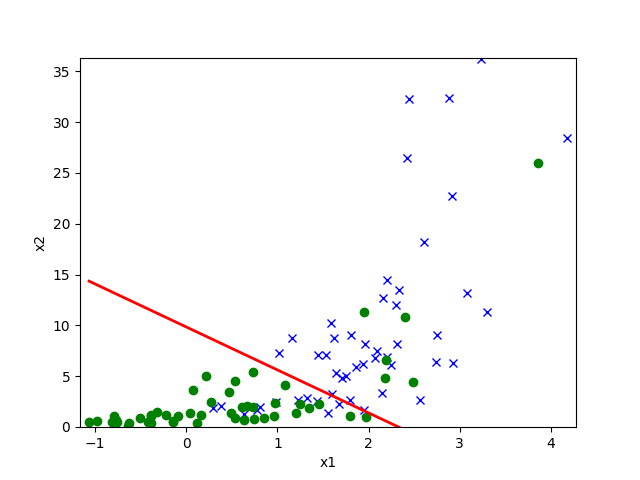
\includegraphics[width=0.45\linewidth]{src/linearclass/logreg_pred_1.png}
%		\caption{Logistic Regression Decision Boundary on Dataset 1}
%	\end{figure}
%
%	\begin{figure}[h]
%		\centering
%		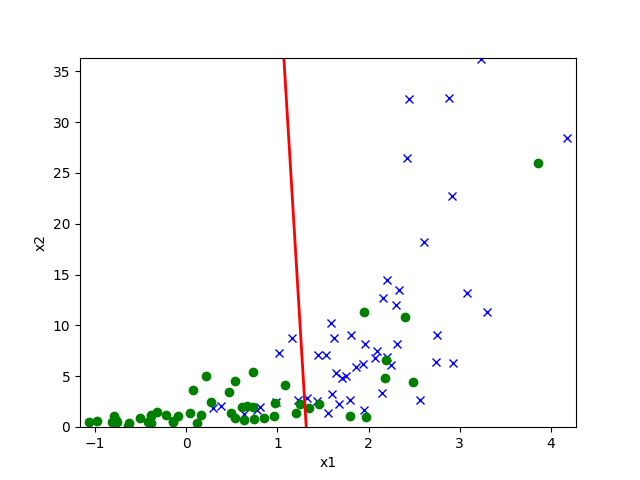
\includegraphics[width=0.45\linewidth]{src/linearclass/gda_pred_1.png}
%		\caption{GDA Decision Boundary on Dataset 1}
%	\end{figure}
%	
	\paragraph{Comment} The decision boundary from logistic regression seems more reasonable. The logistic decision boundary puts weight on both $x_1$ and $x_2$. However, the GDA decision boundary is almost vertical and does not put much weight on $x_2$, the decision is made heavily relied on the $x_1\upi$ for each sample.
	
	\subsection{Question 1(g)}
%	\begin{figure}[h]
%		\centering
%		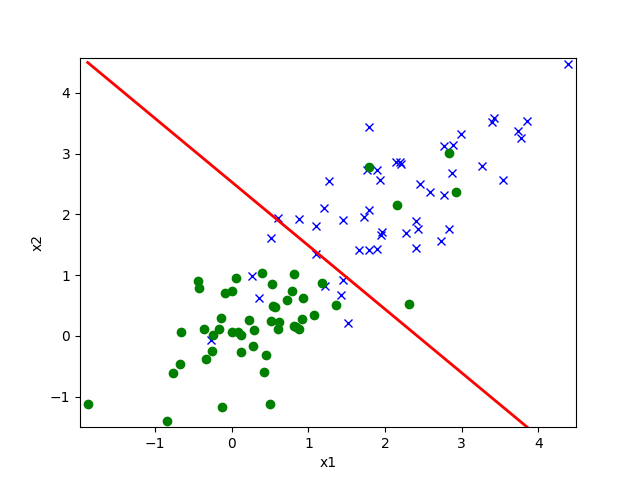
\includegraphics[width=0.45\linewidth]{src/linearclass/logreg_pred_2.png}
%		\caption{Logistic Regression Decision Boundary on Dataset 2}
%	\end{figure}
%
%	\begin{figure}[h]
%		\centering
%		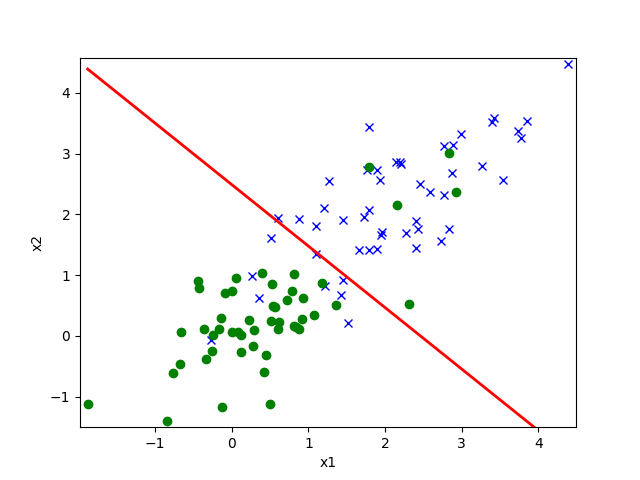
\includegraphics[width=0.45\linewidth]{src/linearclass/gda_pred_2.png}
%		\caption{GDA Decision Boundary on Dataset 2}
%	\end{figure}

	\paragraph{Comment} Decision boundaries from logistic regression and GDA are nearly identical. In the first dataset GDA seem to perform worse than logistic regression. GDA assumed common variance across groups, however, from the scatter plot, the variance of $x_2$ within green dot group is much less the variance of $x_2$ within blue cross group. So the GDA assumption is critically compromised in the first dataset. In contrast, for the second dataset, variance of both $x_1$ and $x_2$ are similar in both groups, the common-covariance assumption of GDA model is more realistic, thus GDA and logistic regression generated similar results on the second dataset.
	
	\subsection{Question 1(h)}
	\paragraph{Comment} we can normalize/standardize $x_1$ and $x_2$ within two groups using 
	\begin{align}
		x\upi_j \leftarrow \frac{x\upi_j - \mu_{x_j}}{\sigma_j}
	\end{align}
	so that both $x_1$ and $x_2$ have variance of (approximately) 1 in both groups, so that the common-covariance assumption of GDA becomes more realistic.
	
	\newpage
	\section{Question 2: Incomplete, Positive-Only Labels}
	\subsection{Question 2(a) Coding}
	\begin{figure}[h]
		\centering
		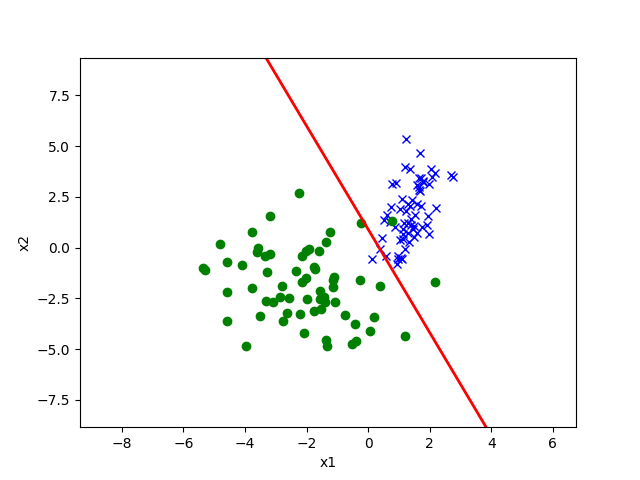
\includegraphics[width=0.6\linewidth]{src/posonly/posonly_true_pred.png}
		\caption{Test Set Prediction of Models Trained on True Label}
	\end{figure}
	
	\subsection{Question 2(b) Coding}
	\begin{figure}[h]
		\centering
		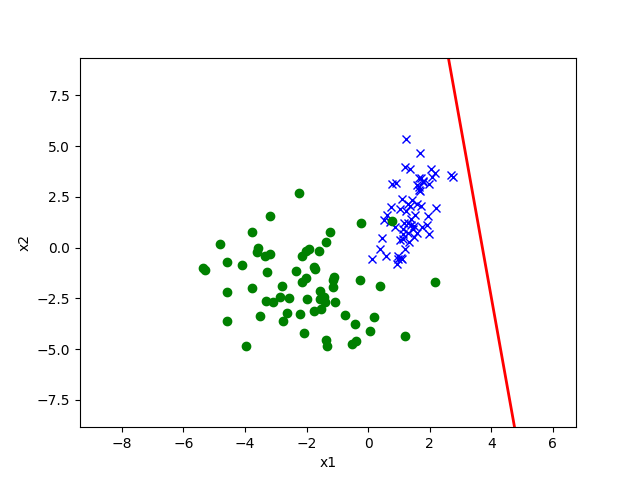
\includegraphics[width=0.6\linewidth]{src/posonly/posonly_naive_pred.png}
		\caption{Test Set Prediction of Naive Model}
	\end{figure}
	
	\subsection{Question 2(c)}
	\begin{proof}
		\begin{align}
			p(t\upi=1 | y\upi=1, x\upi) &= \frac{p(y\upi=1|t\upi=1,x\upi)p(t\upi=1|x\upi)}{p(y\upi=1|x\upi)} \\
			&= \frac{
				p(y\upi=1|t\upi=1,x\upi)p(t\upi=1|x\upi)
			}{
				p(y\upi=1|t\upi=1,x\upi)p(t\upi=1|x\upi)
				+ p(y\upi=1|t\upi=0,x\upi)p(t\upi=0|x\upi)
			} \\
			&= \frac{
				\alpha p(t\upi=1|x\upi)
			}{
				\alpha p(t\upi=1|x\upi) + 0p(t\upi=0|x\upi)
			} \\
			&= \frac{
				\alpha p(t\upi=1|x\upi)
			}{
				\alpha p(t\upi=1|x\upi)
			}=1
		\end{align}
	\end{proof}
	
	\newpage
	
	\subsection{Question 2(d)}
	\begin{proof}
		\begin{align}
			p(t\upi=1|x\upi) &= p(t\upi, y\upi=1|x\upi) + p(t\upi=1, y\upi=0|x\upi) \\
			&= p(t\upi=1|y\upi=1, x\upi) p(y\upi=1|x\upi) \\
			&+ p(y\upi=0|t\upi=1, x\upi) p(t\upi=1|x\upi) \\
			&= 1 p(y\upi=1|x\upi) + (1-\alpha) p(t\upi=1|x\upi) \\
			\implies p(t\upi=1|x\upi) &= \frac{1}{\alpha} p(y\upi=1|x\upi)
		\end{align}
	\end{proof}
	
	\newpage
	
	\subsection{Question 2(e)}
	\begin{proof}
		\begin{align}
			h(x\upi) &= p(y\upi = 1|x\upi) \\
			\implies \expect{h(x\upi)|y\upi=1} &= \expect{p(y\upi = 1|x\upi)|y\upi=1} \\
			&= \mathbb{E}\{
			p(y\upi = 1|t\upi=1, x\upi) p(t\upi=1|x\upi) \\
			&+ p(y\upi = 1|t\upi=0, x\upi) p(t\upi=0|x\upi)
			|y\upi=1
			\} \\
			&= \expect{\alpha p(t\upi=1|x\upi) + 0|y\upi = 1} \\
			&= \alpha \expect{p(t\upi=1|x\upi)|y\upi=1}
		\end{align}
		From part (c), we proved that given $y\upi=1$, $t\upi=1$ with probability 1, conditioned on $x\upi$. Hence,
		\begin{align}
			\expect{p(t\upi=1|x\upi)|y\upi=1} &= 1 \\
			\implies \expect{h(x\upi)|y\upi=1} &= \alpha
		\end{align}
	\end{proof}
	
	\subsection{Question 2(f) Coding}
	\begin{figure}[h]
		\centering
		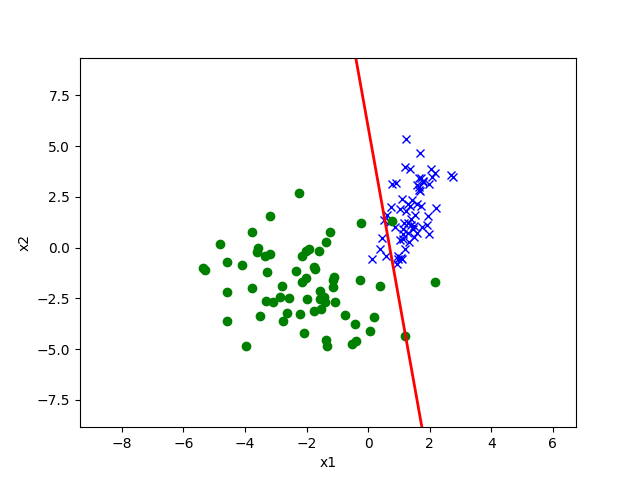
\includegraphics[width=0.6\linewidth]{src/posonly/posonly_adjusted_pred.png}
		\caption{Adjusted Prediction on Test Set}
	\end{figure}
	
	\newpage
	
	\section{Question 3: Poisson Regression}
	\subsection{Question 3(a)}
	\begin{proof}
		\begin{align}
			p(y; \lambda) &= \frac{\exp(-\lambda) \lambda^y}{y!} \\
			&= \exp \log (\frac{\exp(-\lambda) \lambda^y}{y!}) \\
			&= \exp \left (
				- \lambda + y \log (\lambda) - \log(y!)
			\right ) \\
			&= \frac{1}{y!} \exp(\log(\lambda) y - \lambda)
		\end{align}
		therefore, Poisson distribution belongs to the exponential family with
		\begin{align}
			b(y) &:= \frac{1}{y!} \\
			\eta(\lambda) &:= \log(\lambda) \\
			T(y) &:= y \\
			a(\eta) &:= \exp(\eta) = \lambda
		\end{align}
	\end{proof}
	\newpage
	
	\subsection{Question 3(b)}
	\begin{proof}[Answer.]
	\par By definition, the canonical response function maps $\eta$ to the expectation $\expect{T(y); \eta}$, which equals $\expect{y; \eta} = \lambda$ here. Based on the fact that $\eta(\lambda) = \log(\lambda)$, the \ul{exponential} function maps $\eta(\lambda)$ to $\expect{y; \eta}$. Hence, the canonical response function here is the exponential function.
	\end{proof}
	
	\subsection{Question 3(c)}
	\begin{proof}[Derive.]
	\begin{align}
		\pd{}{\theta_j} \log (p(y\upi|x\upi; \theta)) &= \pd{}{\theta_j} 
		\left (\log(b(y)) + \eta^T y\upi - a(\eta) \right )\\
		&= \pd{}{\theta_j} \left (
		\theta^T x\upi y\upi - \exp(\theta^T x\upi)
		\right ) \\
		&= x\upi_j y\upi - \exp(\theta^T x\upi) x\upi_j \\
		&= \left(y\upi - \exp(\theta^T x\upi )\right) x\upi_j
	\end{align}
	The stochastic gradient ascent update rule for parameter $\theta_j$ is 
	\begin{align}
		\theta_j \leftarrow \theta_j + \alpha \left(y\upi - \exp(\theta^T x\upi )\right) x\upi_j
	\end{align}
	where $(x\upi, y\upi)$ is the randomly selected sample, and $\alpha > 0$ denotes the learning rate.
	\end{proof}
	
	\subsection{Question 3(d) Coding}
	\begin{figure}[h]
		\centering
		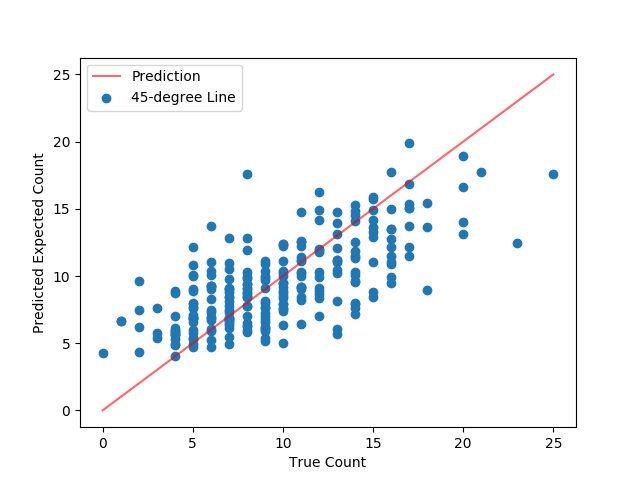
\includegraphics[width=0.6\linewidth]{src/poisson/poisson_pred.png}
		\caption{True Count and Predicted Counts on the Validation Set}
	\end{figure}
	
	\newpage
	\section{Question 4: Convexity of Generalized Linear Models}
	\subsection{Question 4(a)}
	\begin{proof}
		The mean of $y$ is simply
		\begin{align}
			\expect{Y;\eta} &= \int_\R y p(y; \eta)\ dy \\
			&= \int_\R y b(y) \exp(\eta y - a(\eta))\ dy
		\end{align}
		By definition of probability measure, it must be the case that 
		\begin{align}
			\int_\R p(y; \eta)\ dy &= 1
		\end{align}
		for every valid $\eta$. Therefore,
		\begin{align}
			\int_\R b(y) \exp(\eta y - a(\eta))\ dy &= 1 \\
			\implies \int_\R b(y) \exp(\eta y) \frac{1}{\exp(a(\eta))}\ dy &= 1 \\
			\implies \int_\R b(y) \exp(\eta y)\ dy &= \exp(a(\eta)) \\
			\implies \pd{\exp(a(\eta))}{\eta} &= \pd{}{\eta} \int_\R b(y) \exp(\eta y)\ dy \\
			\implies a'(\eta) \exp(a(\eta)) &= \int_\R b(y) \pd{\exp(\eta y)}{\eta}\ dy \\
			\implies a'(\eta) &= \int_\R y b(y) \exp(\eta y) \frac{1}{\exp(a(\eta))}\ dy \\
			\implies a'(\eta) &= \int_\R y b(y) \exp(\eta y - a(\eta))\ dy \\
			&= \expect{Y;\eta}
		\end{align}
	\end{proof}
	
	\newpage
	\subsection{Question 4(b)}
	\begin{proof}
		From part (a),
		\begin{align}
			a'(\eta) &= \int_\R y b(y) \exp(\eta y - a(\eta))\ dy \\
			\implies \frac{\partial^2 a(\eta)}{\partial \eta^2} &= \pd{}{\eta} \int_\R y b(y) \exp(\eta y - a(\eta))\ dy \\
			&= \int_\R y b(y) \exp(ny - a(\eta)) \left (
				y - a'(\eta)
			\right)\ dy \\
			&= \int_\R y^2 b(y) \exp(ny - a(\eta))\ dy - a'(\eta) \int_\R y b(y) \exp(ny - a(\eta))\ dy \\
			&= \expect{Y^2; \eta} - a'(\eta) \expect{Y; \eta} \\
			&= \expect{Y^2; \eta} - \expect{Y; \eta}^2 \\
			&= \var{Y; \eta}
		\end{align}
	\end{proof}
	
	\newpage
	\subsection{Question 4(c)}
	\begin{proof}
		
	\end{proof}
	
	\newpage
	\section{Question 5: Linear Regression}
	\subsection{Question 5(a)}
	\begin{align}
		J(\theta) &:= \frac{1}{2} \sum_{i=1}^n \left(y\upi - \theta^T \phi(x\upi) \right)^2 \\
		\theta &\leftarrow \theta + \alpha \sum_{i=1}^n \left(y\upi - \theta^T \hat{x}\upi \right) \hat{x}\upi
	\end{align}
	where $\alpha$ denotes the learning rate.
	\subsection{Question 5(b) Coding}
	\paragraph{Comment} It is theoretically possible to fit a sine function using polynomials by Taylor's expansion. However, when $k=3$, the polynomial model is not expressive enough to capture all curvatures in the training set.
	\begin{figure}[h]
		\centering
		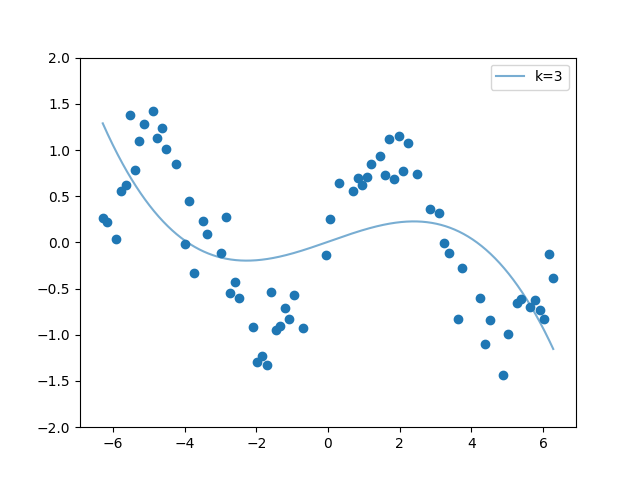
\includegraphics[width=0.6\linewidth]{src/featuremaps/5b.png}
		\caption{Polynomial Features up to Degree 3}
	\end{figure}
	
	\newpage
	\subsection{Question 5(c) Coding}
	\paragraph{Comment} For models with $k=5$ or $k=10$, the model captures the curvature of training samples much better than $k=3$ model does. However, for $k=20$, the model starts to over fit the noise in the training set, and the expected value demonstrates abnormal curvature near $x=-3$, $x=4.5$, and $x=6$.
	\begin{figure}[h]
		\centering
		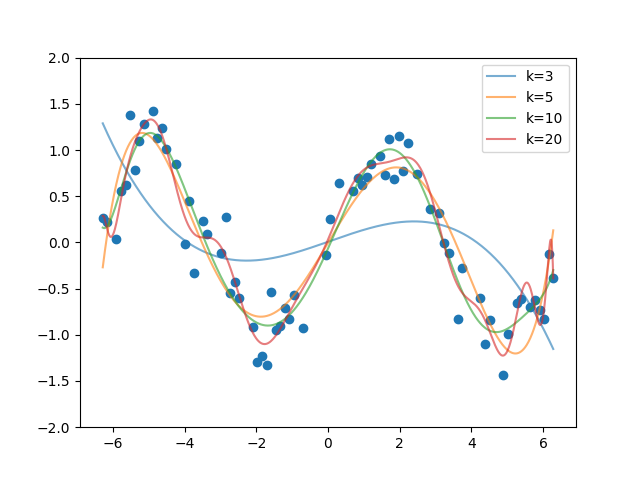
\includegraphics[width=0.6\linewidth]{src/featuremaps/5c.png}
		\caption{Polynomial Features}
	\end{figure}
	
	\subsection{Question 5(d) Coding}
	\paragraph{Comment} By observing the training set, it can be postulated that the true data generating process actually involves a sin function. Adding the $\sin(x)$ feature allows the model to fully capture the underlying pattern, even with low degree of polynomial terms. Also, when $k$ is large, the model starts to over fit training samples by capturing the noise.
	\begin{figure}[h]
		\centering
		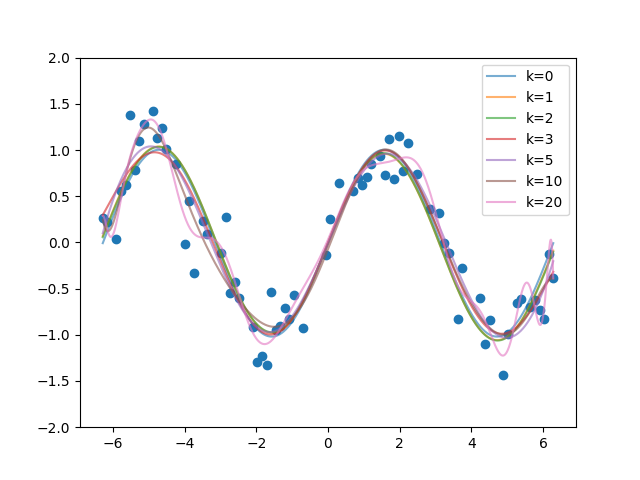
\includegraphics[width=0.6\linewidth]{src/featuremaps/5d.png}
		\caption{Polynomial and Sin Features}
	\end{figure}
	
	\newpage
	\subsection{Question 5(e) Coding}
	\begin{figure}[h]
		\centering
		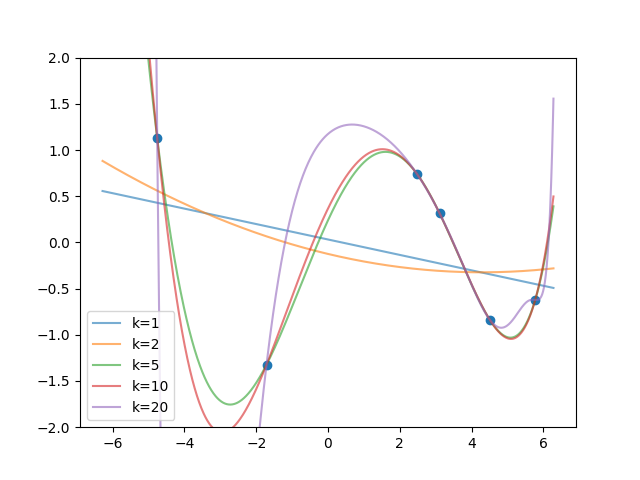
\includegraphics[width=0.6\linewidth]{src/featuremaps/5e.png}
		\caption{Overfitting on Small Dataset}
	\end{figure}
	\paragraph{Comment} When the number of features is smaller than number of training samples, the model is experiencing under fitting problem. However, when the number of parameters in the model is more than the number of training, the model can fit all training samples exactly (when $k \geq 5$, the fitting line passes through all training samples precisely), and the model suffers from over fitting problem.
\end{document}









